% Teilaufgabe 3

\newpage
\section{Herleitung des Reflexionsgrads $R$}
\label{sec:reflexionsgrad}

\subsection{Fresnel-Formeln}
\label{sub:fresnel}
Trifft eine elektromagnetische Welle senkrecht (y-Richtung) auf ein optisches Medium (x-z-Ebene), wird diese gebrochen und reflektiert. Dabei entstehen drei ebene Wellen die einfallende Welle mit Index e, die reflektierte Welle  mit Index r und die gebrochene Welle mit Index g mit der Gleichung für die elektrische Feldstärke $\vec{E}$:
\begin{gather}
	\vec{E}_i = \vec{A}_i \cdot e^{i(\omega_i t - \vec{k}_i\vec{r})};~i = \mathrm{e,~r,~g},
	\label{eq:efeld}
\end{gather}
wobei $\vec{A}_i$ die Amplitudenvektor der Welle, $\omega_i$ die Frequenz, $\vec{k}_i$ der Wellenvektor und $\vec{r}$ der Richtungsvektor ist. Es gilt des weiteren, dass die Tangentialkomponenten von $\vec{E}$ stetig an der Grenzfläche ($\vec{r} = 0$) ist, wodurch folgt:
\begin{gather}
	E_{et} + E_{rt} = E_{gt} \Rightarrow A_{et} e^{i\omega_e t} + A_{rt} e^{i\omega_r t} = A_{gt} e^{i\omega_g t};~t = \mathrm{x,~z}
	\label{eq:tangentialKomp}
\end{gather} 
Die Gleichung \ref{eq:tangentialKomp} hat für beliebige Zeiten $t$ nur dann nicht-triviale Lösung, wenn:
\begin{gather}
	\omega_e = \omega_r = \omega_g,
	\label{eq:frequenzRelation}
\end{gather}
gilt. Daraus folgt für die tangential Komponenten:
\begin{gather}
	A_{et} + A_{rt} = A_{gt};~t = \mathrm{x,~z}~.
	\label{eq:ampRelation}
\end{gather}
\begin{center}
	\captionsetup{type=figure}
	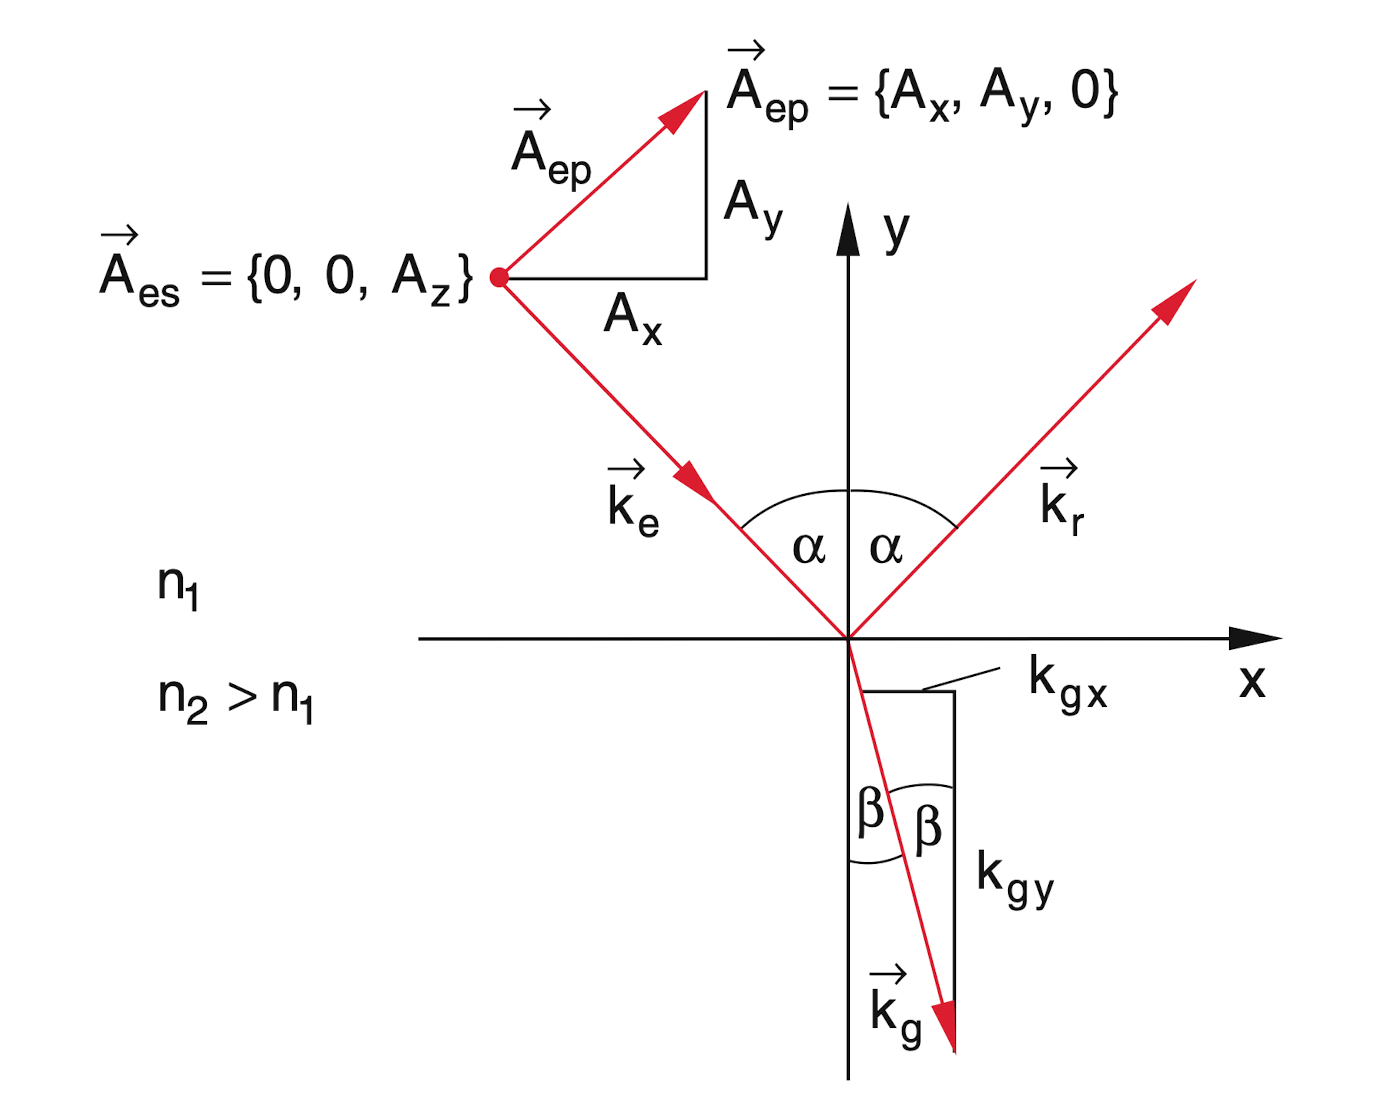
\includegraphics[width=0.6\textwidth]{Fresnel.png}
	\captionof{figure}{Darstellung der Geometrie zur Herleitung der Fresnel-Gleichung. Komponente $A_{\mathrm{es}}$ steht senkrecht zur Zeichenebene. \cite{DemtroederOptik}}
	\label{fig:reflexion}
\end{center}
Die Vektoren lassen sich für diesen Sachverhalt in zwei Komponenten zerlegen. In einen Parallelkomponente mit Index p, welche die Koordinaten x und y enthält und eine senkrechten Komponente mit Index s, welche die Koordinate z beinhaltet, siehe Abb. \ref{fig:reflexion}. Aus Gleichung \ref{eq:ampRelation} folgt für die senkrechte Komponente an der Grenzfläche:
\begin{gather}
	A_{es} + A_{rs} = A_{gs}.
	\label{eq:ampsenkRelation}
\end{gather}
Betrachtet man nun die Tangentialkomponente der magnetischen FLussdichte $\vec{B}$ und setzt die Stetigkeit dieser Komponente voraus, folgt aus der Relation
\begin{gather}
	\vec{B} = \frac{1}{\omega} \left( \vec{k} \times \vec{E} \right),
	\label{eq:bfeldRelation}
\end{gather}
dass
\begin{gather}
	\left( \vec{k}_e \times \vec{E}_e \right)_x + \left( \vec{k}_r \times \vec{E}_r \right)_x = \left( \vec{k}_g \times \vec{E}_g \right)_x~,\\[0.2cm]
	\Rightarrow k_{ey}A_{es} + k_{ry}A_{rs} = k_{gy}A_{gs} \\[0.2cm]
	\xrightarrow{k_{ry} = -k_{ey}} A_{es} + A_{rs} = \frac{k_{gy}}{k_{ey}}A_{gs} = a A_{gs};~\mathrm{mit}~a=\frac{k_{gy}}{k_{ey}}
	\label{eq:ampsenkwaveRelation}
\end{gather}
Aus Gleichung \ref{eq:ampsenkRelation} und Gleichung \ref{eq:ampsenkwaveRelation}  erhält man:
\begin{gather}
	\frac{A_{rs}}{A_{es}} = \frac{1-a}{1+a}~~~~~\frac{A_{gs}}{A_{es}} = \frac{2}{1+a}~.
	\label{eq:ampsenktotalRelation}
\end{gather}
Aus Abb. \ref{fig:reflexion} entnimmt man die Relation:
\begin{gather}
	\frac{k_{ey}}{k_e} = \cos\alpha~~~~~\frac{k_{gy}}{k_g} = \cos\beta~.
	\label{eq:wavetriRealation}
\end{gather}
Zusammen mit $k_g = \frac{n_2}{n_1}k_e$ ergibt sich:
\begin{gather}
	\frac{k_{gy}}{k_{ey}} = \frac{k_g\cos\beta}{k_e\cos\alpha} = \frac{n_2\cos\beta}{n_1\cos\alpha} = a ~.
	\label{eq:yverhaeltnis}
\end{gather}
Zuletzt setzt man nun Gleichung \ref{eq:yverhaeltnis} in Gleichung \ref{eq:ampsenktotalRelation} und erhält:
\begin{gather}
	\boxed{
	\begin{aligned}
		\rho_s &= \frac{A_{rs}}{A_{es}} &= \frac{n_1\cos\alpha - n_2\cos\beta}{n_1\cos\alpha + n_2\cos\beta}\\
		\tau_s &= \frac{A_{gs}}{A_{es}} &= \frac{2n_1\cos\alpha}{n_1\cos\alpha + n_2\cos\beta}
	\end{aligned}
	}
	\label{eq:fresnelsenk}
\end{gather}
Analoge Überlegungen ergeben für die parallelen Komponenten:
\begin{gather}
	\boxed{
	\begin{aligned}
		\rho_p &= \frac{A_{rp}}{A_{ep}} &= \frac{n_2\cos\alpha - n_1\cos\beta}{n_2\cos\alpha + n_1\cos\beta}\\
		\tau_p &= \frac{A_{gp}}{A_{ep}} &= \frac{2n_1\cos\alpha}{n_2\cos\alpha + n_1\cos\beta}
	\end{aligned}
	}
	\label{eq:fresnelpar}
\end{gather}
Hierbei handelt es sich bei $\rho$ um den \textbf{Reflexionskoeffizient} und bei $\tau$ um den \textbf{Transmissionskoeffizient}, welche das Amplitudenverhältnis für die gebrochene und reflektierte Welle angeben.
Zusammen ergeben Gleichungen \ref{eq:fresnelsenk} und \ref{eq:fresnelpar} die \textbf{Fresnel-Formeln}. \cite{DemtroederOptik}

\subsection{Der Reflexionsgrad $R$}
Der Reflexionsgrad $R$ ist definiert als das Verhältnis aus reflektierter Intensität $I_r$ und einfallender Intensität $I_e$ :
\begin{gather}
	R = \frac{I_r}{I_e} = \left( \frac{A_r}{A_e} \right)^2 ~.
	\label{eq:refexionsgrad}
\end{gather} 
Zusammen mit den Fresnel-Formeln \ref{eq:fresnelsenk} und \ref{eq:fresnelpar} ergibt sich:
\begin{gather}
	R_s = \left( \frac{n_1\cos\alpha - n_2\cos\beta}{n_1\cos\alpha + n_2\cos\beta} \right)^2\\
	R_p = \left( \frac{n_2\cos\alpha - n_1\cos\beta}{n_2\cos\alpha + n_1\cos\beta} \right)^2
	\label{eq:refexionsgradfresnel}
\end{gather}
Für eine senkrecht einfallende Welle ($\alpha = 0$) und der Bedingung \ref{eq:brechung} aus Kapitel \ref{sec:interferenz} folgt für den Reflexionsgrad, dass senkrechte und parallele Komponente gleich sind und damit:
\begin{gather}
	\boxed{R(\alpha=0) = \left( \frac{n_1- n_2}{n_1 + n_2} \right)^2}
	\label{eq:reflexionsgradsenk}
\end{gather}
Nimmt man nun an, dass das Medium außerhalb Luft ($n_1=1$) und der Brechungsindex des Materials $n_2 = n + i\kappa$ folgt daraus für Gleichung \ref{eq:reflexionsgradsenk}:
\begin{gather}
	\boxed{R = \left| \frac{(1 - n) -i\kappa}{(1 + n) +i\kappa} \right|^2 = \frac{(1 - n)^2 + \kappa^2}{(1 + n)^2 + \kappa^2}}
\end{gather}